\documentclass[a4paper,11pt,oneside]{article}

\usepackage{amsmath,amssymb,epsfig}
\usepackage[T1]{fontenc}
\usepackage{ae,aecompl}
\usepackage{epsfig}
\usepackage{subfigure}
\usepackage{url}
\addtolength{\voffset}{-1cm}
\addtolength{\hoffset}{-1cm}
\setlength{\parindent}{0in}
\addtolength{\textwidth}{1.8cm}
\addtolength{\textheight}{1cm}
\addtolength{\parskip}{.5cm}

% Example definitions.
% --------------------
\def\e{{e^{j\omega}}}
\def\W{{W_M}}
\def\sumk{{\sum_{k=-\infty}^{\infty}}}
\def\x{{\mathbf x}}
\def\X{{\mathbf X}}
\def\Y{{\mathbf Y}}
\def\u{{\mathbf u}}
\def\U{{\mathbf U}}
\def\x{{\mathbf x}}
\def\s{{\mathbf s}}
\def\A{{\mathbf A}}
\def\y{{\mathbf y}}
\def\w{{\mathbf w}}
\def\B{{\mathbf B}}
\def\a{{\mathbf a}}
\def\D{{\mathbf D}}
\def\P{{\mathbf P}}
\def\n{{\mathbf n}}
\def\V{{\mathbf V}}
\def\R{{\mathbf R}}
\def\I{{\mathbf I}}
\def\M{{\mathbf M}}
\def\sech{{\mathrm{sech}}}
\def\L{{\cal L}}
\def\Cum{{\rm{Cum}}}
\def\var{{\rm{var}}}
\def\T{{\mathbf T}}
\def\C{{\mathbf C}}
\def\tf{{\emph{t-f}}}


% Title.
% ------
\title{\large{\textbf{EXERCISE 2}}}
\author{SGN-1156 Signal Processing Techniques\\
\texttt{http://www.cs.tut.fi/courses/SGN-1156}\\
Tampere University of Technology\\
Germ\'an G\'omez-Herrero, \url{http://germangh.com}}
\date{November 11, 2009}


\begin{document}

\maketitle



%%%%%%%%%%%%%%%%%%%%%%%%%%%%%%%%%%%%%%%%%%%%%%%%%%%%%%%%%%%%%%%
\textbf{PROBLEM 1:} Determine the DTFT of each of the following sequences:

\begin{itemize}
\item[(a)] $x_a[n] = \mu[n]-\mu[n-5]$
\item[(b)] $x_b[n] = \alpha^n\left(\mu[n]-\mu[n-8]\right) \qquad |\alpha|< 1$
\item[(c)] $x_c[n] = (n+1)\alpha^n\mu[n] \qquad |\alpha|<1$
\end{itemize}  



\vspace{1cm}
%%%%%%%%%%%%%%%%%%%%%%%%%%%%%%%%%%%%%%%%%%%%%%%%%%%%%%%%%%%%%%%




%%%%%%%%%%%%%%%%%%%%%%%%%%%%%%%%%%%%%%%%%%%%%%%%%%%%%%%%%%%%%%%
\textbf{PROBLEM 2: (problem 3.41 from the book)} Let $G_1(e^{j\omega})$ denote the discrete-time Fourier transform of the sequence $g_1[n]$ shown in the figure below. Express the DTFTs of $g_2[n]$, $g_3[n]$ and $g_4[n]$ in terms of $G_1(e^{j\omega})$. Do not evaluate $G_1(e^{j\omega})$.


\begin{figure}[ht!]
\centering
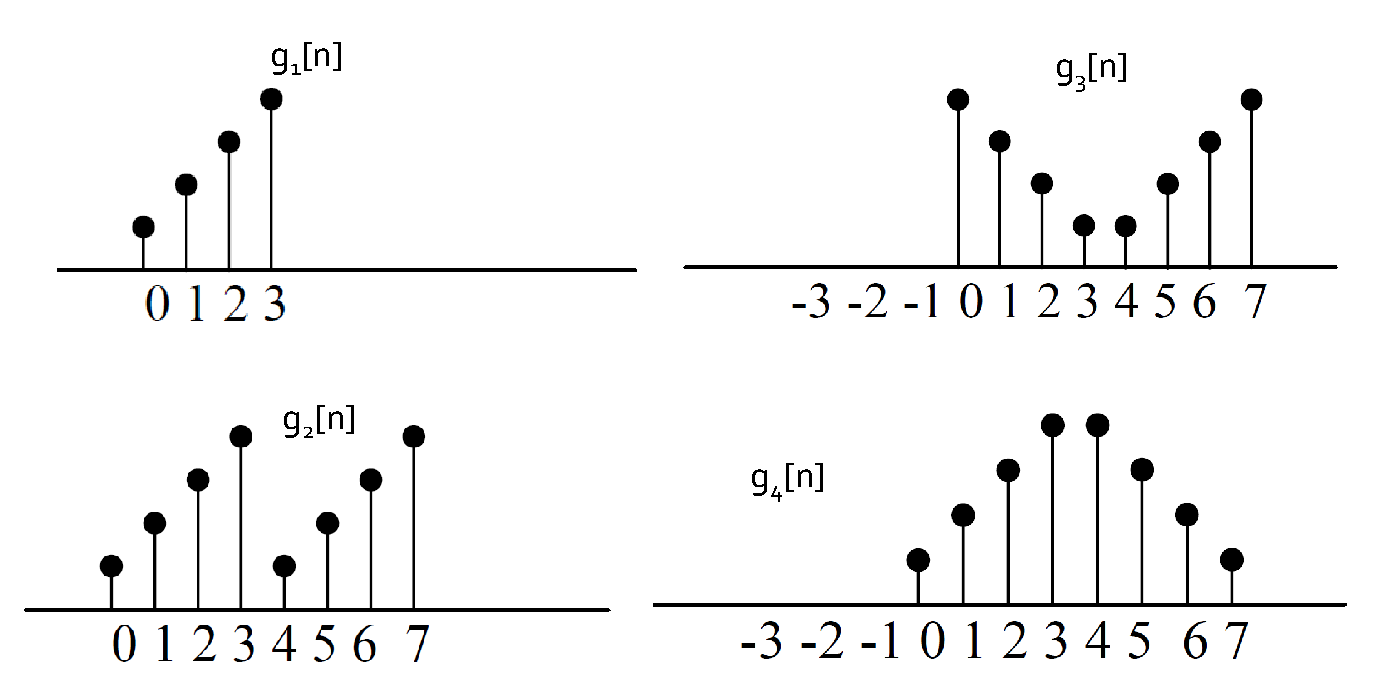
\includegraphics[width=.8\textwidth]{fig4.eps}
\end{figure}


\vspace{1cm}
%%%%%%%%%%%%%%%%%%%%%%%%%%%%%%%%%%%%%%%%%%%%%%%%%%%%%%%%%%%%%%%



%%%%%%%%%%%%%%%%%%%%%%%%%%%%%%%%%%%%%%%%%%%%%%%%%%%%%%%%%%%%%%%
\textbf{PROBLEM 3: (problem 3.34 from the book)} Let $X(e^{j\omega})$ denote the DTFT of a complex sequence $x[n]$. Determine the DTFT $Y(e^{j\omega})$ of the sequence $y[n]=x[n]\ast x^*[-n]$ in terms of $X(e^{j\omega})$, and show that it is a real-valued function of $\omega$.


\vspace{1cm}
%%%%%%%%%%%%%%%%%%%%%%%%%%%%%%%%%%%%%%%%%%%%%%%%%%%%%%%%%%%%%%%



%%%%%%%%%%%%%%%%%%%%%%%%%%%%%%%%%%%%%%%%%%%%%%%%%%%%%%%%%%%%%%%
\textbf{PROBLEM 4:}  Consider the following interconnection of linear shift-invariant systems:

\begin{figure}[ht!]
\centering
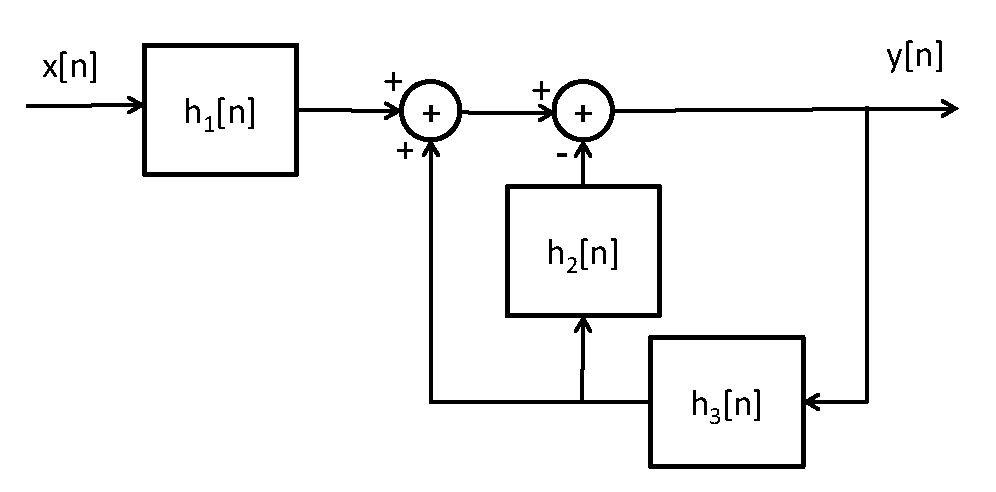
\includegraphics[width=.7\textwidth]{fig1.eps}
\end{figure}

Express the frequency response of the overall system $H(e^{j\omega})$ in terms of the frequency responses of the subsystems $H_1(e^{j\omega})$, $H_2(e^{j\omega})$, and $H_3(e^{j\omega})$.

\vspace{1cm}

%%%%%%%%%%%%%%%%%%%%%%%%%%%%%%%%%%%%%%%%%%%%%%%%%%%%%%%%%%%%%%%




%%%%%%%%%%%%%%%%%%%%%%%%%%%%%%%%%%%%%%%%%%%%%%%%%%%%%%%%%%%%%%%
\textbf{PROBLEM 5.} Consider the following interconnection of LTI systems:

\begin{figure}[ht!]
\centering
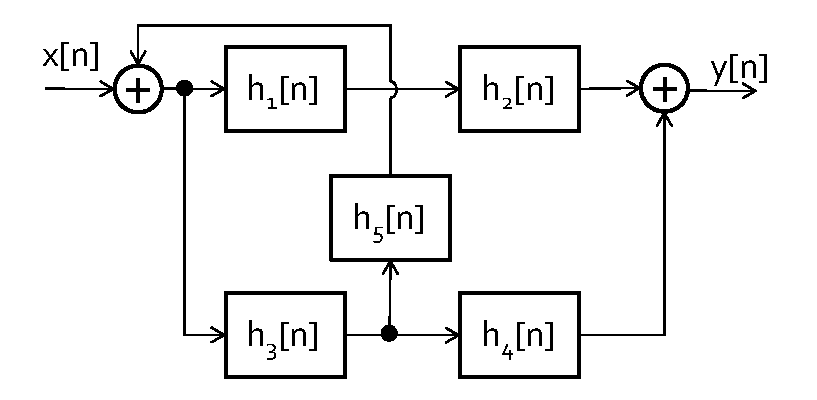
\includegraphics[width=.7\textwidth]{fig3.eps}
\end{figure}

Express the frequency response of the overall system $H(e^{j\omega})$ in terms of the frequency responses of the subsystems depicted in the diagram.

\vspace{1cm}
%%%%%%%%%%%%%%%%%%%%%%%%%%%%%%%%%%%%%%%%%%%%%%%%%%%%%%%%%%%%%%%
 

%%%%%%%%%%%%%%%%%%%%%%%%%%%%%%%%%%%%%%%%%%%%%%%%%%%%%%%%%%%%%%%
\textbf{PROBLEM 6.} Consider the interconnection of linear shift-invariant systems in the figure below:



\begin{figure}[h!]
\centering
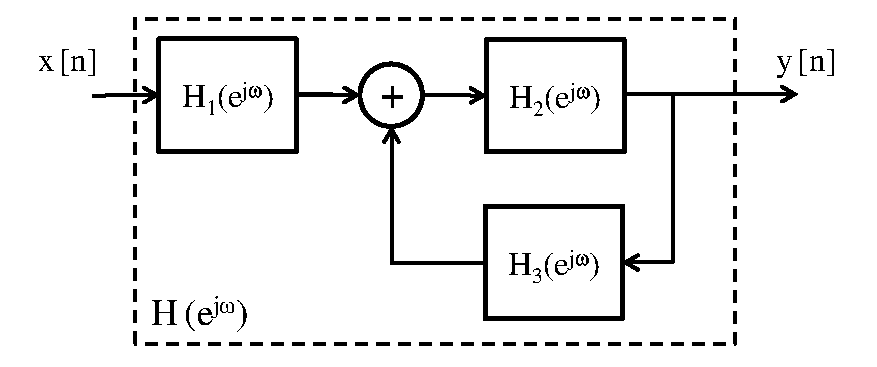
\includegraphics[width=.7\textwidth]{fig5.eps}
\end{figure}



\begin{itemize}
\item[(a)] Express the frequency response of the overall system $H(e^{j\omega})$ in terms of the frequency responses of the subsystems $H_1(e^{j\omega})$, $H_2(e^{j\omega})$ and $H_3(e^{j\omega})$.
\item[(b)] Determine the frequency response $H(e^{j\omega})$ of the overall system if:
\[
\begin{array}{lll}
h_1[n] &=& \frac{\sin(\frac{\pi}{3}n)}{\pi n}\\
h_2[n] &=&(0.3)^{n}\mu[n]\\
h_3[n] &=&\delta[n-2]
\end{array}
\]
\end{itemize}


\vspace{1cm}
%%%%%%%%%%%%%%%%%%%%%%%%%%%%%%%%%%%%%%%%%%%%%%%%%%%%%%%%%%%%%%%
 


%%%%%%%%%%%%%%%%%%%%%%%%%%%%%%%%%%%%%%%%%%%%%%%%%%%%%%%%%%%%%%%
\textbf{PROBLEM 7 (problem 3.59 from the book):} An LTI IIR discrete-time system is described by the difference equation
\[
y[n] + a_1y[n-1] = b_0x[n]+b_1x[n-1]
\]
where the input is $x[n]$, the output is $y[n]$, and the constants $a_1$, $b_0$ and $b_1$ are real. Determine the expression for its frequency response. For what values of $b_0$ and $b_1$ will the magnitude response be a constant for all values of $\omega$?.




\vspace{1cm}
%%%%%%%%%%%%%%%%%%%%%%%%%%%%%%%%%%%%%%%%%%%%%%%%%%%%%%%%%%%%%%%




%%%%%%%%%%%%%%%%%%%%%%%%%%%%%%%%%%%%%%%%%%%%%%%%%%%%%%%%%%%%%%%
\textbf{PROBLEM 8:} Consider the system defined by the difference equation 

\[
y[n] = ay[n-1]+bx[n]+x[n-1]
\]

where $a$ and $b$ are real, and $|a|<1$. Find the relationship between $a$ and $b$ that must exist if the frequency response is to have a constant magnitude for all $\omega$, that is $|H(e^{j\omega})|=1$.
\vspace{1cm}
%%%%%%%%%%%%%%%%%%%%%%%%%%%%%%%%%%%%%%%%%%%%%%%%%%%%%%%%%%%%%%%




\end{document}